\documentclass[10pt,twocolumn]{article}
\title{Convolutional Neural Networks for Classifying Handwritten Digits}
\date{December 5, 2014}
\author{
	Favyen Bastani \\
	fbastani@perennate.com
	\and
	Zhengli Wang \\
	wzl@mit.edu
}

\usepackage[margin=1in]{geometry}
\usepackage{graphicx}
\usepackage{amsmath}
\usepackage{subcaption}
\usepackage{cite}
\usepackage[colorlinks]{hyperref}
\usepackage{placeins}
\setlength{\columnsep}{3em}

\begin{document}

\maketitle

\begin{abstract}
In this project, we implement a CPU-based convolutional neural network (CNN) library in Python, using the \texttt{numpy} library for fast array operations. Our library constructs the complex structure of the CNN, performs forward propagation and pooling, and trains the network using backward propagation and stochastic gradient descent. We evaluate CNN performance in terms of classification accuracy and training time on the MNIST database under a wide range of network parameters, and compare CNN to feature extraction approaches such as HOG. We find that CNN is able to achieve much lower misclassification rate (as low as 1.73\%), but requires significantly more time for training of features.
\end{abstract}

\section{Introduction} \label{sec:introduction}

Image recognition algorithms have become pervasive: on Google Maps Street View, image recognition protects privacy by automatically blurring faces and license plate numbers \cite{streetview}; robots use object recognition to autonomously move or assemble structures; meanwhile, individuals routinely employ optical character recognition for scanning documents and facial recognition for labeling photographs. Over the last decade, image recognition approaches have developed dramatically. Initially, feature extraction techniques such as HOG and FAST were typically combined with support vector machine (SVM) classifiers, with research often focusing on selection of SVM kernels and defining features for specific image types. Recently, though, neural networks have received renewed attention and achieved high classification performance.

Cells in the mammalian visual cortex are able to identify local patterns in the visual field \cite{website:lenet}. Convolutional neural networks (CNNs) aim to do the same through \emph{convolutional and pooling layers}. While traditional neural networks are composed of densely connected layers, where each neuron in the previous layer connects to each neuron in the next layer, convolutional layers restrict filters to be applied on local sub-regions of an input image. By training these layers through back-propagation, these filters eventually detect specific features in the image that help with classification. CNNs have achieved high image recognition accuracy on a large number of datasets, including ImageNet (for object recognition) \cite{imagenet}, face recognition \cite{facerec}, and video quality assessment \cite{videoquality}.

In this project, we implement a fast CPU-based CNN toolkit \cite{git:cnn} in Python, and apply it to the MNIST handwritten digits database \cite{mnist}. We evaluate the performance of various neural network parameters (including layer configuration, output layer activation function, and training algorithm) in terms of classification accuracy and training speed, and compare CNN to feature extraction approaches. We find that while CNNs require significantly more training time, they outperform other algorithms with minimal tuning of the network.

In Sections \ref{sec:neural} and \ref{sec:cnn}, we detail convolution and pooling functions, the convolutional neural network structure and training algorithm, and our implementation. In Section \ref{sec:evalcnn}, we experiment with various neural network parameters, and in Section \ref{sec:evalfeature}, we compare with SVM-based algorithms. Finally, we conclude in Section \ref{sec:conclude}.

\section{Neural networks} \label{sec:neural}

An artificial neural network (ANN) consists of neuron units that, when composed in a layered network, compute some output function from an input vector $y = h(x)$. Each neuron in the network has a specific set of input values (which may be elements of the input vector of the network, or outputs from other neurons) and a single output. The output is generally computed as $n_{w, b}(z) = f(w \cdot z + b)$ for some \emph{activation function} $f$, weight vector $w$, and bias parameter $b$. The sigmoid function is often used as the activation function, i.e. $f(l) = \frac{1}{1+e^{-l}}$, because it mimics the hard threshold activation pattern of a biological neuron.

Neurons are connected to form a neural network. Typically, the network is composed of layers of neurons, where neurons in the first layer accept inputs from the input vector $x$, and neurons in each following layer take inputs from the outputs of the neurons in the preceding layer. Then, the network output vector $y$ consists of the outputs from neurons in the last layer of the network. In fully connected neural networks, a neuron takes inputs from every neuron in the previous layer.

Forward propagation refers to the process of propagating some input vector $x$ through each layer of the neural network to compute $y = h(x)$. In a fully connected neural network, this can be done using efficient matrix operations (which can take advantage of fast matrix libraries such as \texttt{numpy}). Let $Z_l$ be the output vector of the $l$th neural network layer (where $Z_0 = x$) and $n_{li}$ be the $i$th neuron in layer $l$; then, $Z_{l+1} = f(W^{\text{T}} Z_l + B)$ where $W_{ij}$ is the weight from $n_{li}$ to $n_{l+1,j}$ and $B_j$ is the bias parameter for neuron $n_{l+1,j}$.

Neural networks can be trained using back propagation. At a high level, we compute a cost function on the outputs from the neural network given some input and desired output, and propagate the error (in the form of partial derivatives of the cost) starting at the last layer to the first layer. These error terms are then used to compute the derivative with respect to specific weight and bias parameters, which can then be updated via gradient descent.

\subsection{ANN for multi-label classification}

Artificial neural networks are often used for multi-label classification. However, the sigmoid activation function is not well suited for this purpose, where we want to assign exactly one label $c$ for each input vector $x$. Instead, we use \emph{softmax activation function}, defined as

$$f(L, i) = \frac{e^{L_i}}{\sum_j e^{L_j}}$$

Here, $L$ is a vector containing inputs to the activation function for each neuron in the softmax layer. For back propagation, the cost function given a desired output vector $o$ is the cross-entropy error function \cite{multilabelerror},

$$E = -\sum_i o_i \text{log}(y_i)$$

\subsection{Stochastic gradient descent} \label{subsec:SGD}

In normal gradient descent neural network training, we iteratively update parameters (weights and bias terms) after averaging derivatives from back propagation across all training samples. However, when the training set is large, each iteration of gradient descent may take a significant amount of time to complete. Stochastic gradient descent instead randomly selects mini-batches of a predetermined size from the training samples on each iteration and updates parameters by averaging derivatives across only the selected samples (the batch size is generally selected to yield optimal performance with matrix libraries, although in our implementation we perform back propagation separately for each sample). This increases solution sparsity as well as convergence speed.

We implement one variation of stochastic gradient descent that further reduces training time in many cases. Rather than updating parameters directly from the computed gradient $\nabla$, we apply a momentum that retains gradients from previous iterations. Let $v_0 = 0$ be the initial velocity. For a training rate $\alpha$ and momentum $m$, we update parameters $\theta_i$ on the $i$th iteration as \cite{ufldl}

$$v_i = mv_{i-1} + \alpha \nabla_i$$
$$\theta_i = \theta_{i-1} - v_i$$

Note that the training rate $\alpha$ is generally smaller in stochastic gradient descent than in conventional gradient descent because the random mini-batch selection introduces greater variance on the training process.

\section{Convolutional neural networks} \label{sec:cnn}

Images, along with many other data types such as audio signals, exhibit strong local patterns that need to be identified for classification. In some cases, fully connected neural networks may ignore these patterns, perhaps overfitting instead; in other cases, training fully connected networks to identify local patterns and achieve high classification accuracy takes a significant number of training iterations. Convolutional neural networks take an alternate approach, where the localized pattern properties are directly encoded into the structure of the neural network. In this section, we discuss the functionality of convolution and pooling layers, and strategies for incorporating them into neural networks.

\subsection{Convolution}

Images can often be hierarchically broken down into features and sub-features that support image recognition. For example, a flower may contain a stem and a petal, each of which consist of edges at various positions and angles. Additionally, these features may exist at various locations in the image: if an image is shifted in one direction, an image recognition algorithm should still be able to classify it in the same way.

The idea behind convolutional layers for image recognition is that a feature can be represented as an $n$ by $n$ \emph{filter}, and then convolved two-dimensionally with the $m$ by $m$ input (which in this case would be an image). If regions of the input match up with the filter, then elements of the convolution output corresponding to those regions will generally take higher values. The output from the convolution is added with a bias term and passed through an activation function. Notably, each component of the convolution can be modeled as a neuron: each neuron takes inputs from a sub-region, multiplies the input by a weight matrix (the filter), and then applies the activation function; besides the sparsely connected input, the only other difference from conventional neural networks is that we require the weight matrix to be the same across multiple neurons (since convolution applies a single filter repeatedly across the image). This enables the detection of local patterns that we desire, since the filter is restricted to only consider sub-regions of the input, while still incorporating the weights and bias components that define neural networks.

In each convolutional layer, we have $k$ filters, each an $n$ by $n$ matrix. Then, for an $m$ by $m$ input, we get a $k$ by $(m - n + 1)$ by $(m - n + 1)$ output from the two-dimensional convolution.

\subsection{Pooling}

Pooling layers apply an aggregate function (typically either max or mean) on non-overlapping regions of the output from convolutional layers (this is done separately for each filter). These regions are often equal in size; so if the output from the convolutional layer is 30 by 30, the pooling layer may pool across each of the four 15 by 15 regions, yielding four output values.

Pooling accomplishes two purposes. First, we reduce the amount of data that later layers need to consider, speeding up training and reducing overfitting. Second, we get a degree of translation invariance. If the input is shifted slightly, the result after pooling will still be similar. This is desirable since generally image recognition classes should remain the same under basic transforms.

\subsection{Network}

Convolution and pooling can be used in isolation, without incorporation in a convolutional neural network. In this case, an autoencoder is typically used to train the filters, where the training goal is to have the output layer match the input layer despite a smaller number of neurons in intermediate layers. The trained filters can then be used to extract features from both training and testing data, and then fed into any classifier. This also supports unsupervised learning of features.

Convolutional neural networks present a more interesting case, where the convolution and pooling operations are combined with classification into a single structure that can be trained in one process. Typical convolutional neural networks consist of one to three convolutional layers followed by fully connected hidden layers; back propagation is carried out across the entire network. When there are several convolutional layers, the first convolutional layer often is used by the network as an edge detector (this determination happens from training alone, without any manual specification other than the layer sizes), while later convolutional layers in the network detect more and more complex features; for simple datasets, a single convolutional layer can be applied to directly identify features. The hidden layers use final pooling outputs to eventually classify the image.

\section{Experimental setup} \label{sec:evalcnn}

We implement a CPU-based convolutional neural network library \cite{git:cnn} in Python using the \texttt{numpy} package, which provides fast scientific computing operations. Our implementation includes a \texttt{Network} class which has attributes that represent the number of layers and the number of neurons in each layer. Our code can use either ``softmax'' or ``sigmoid'' activation functions of neurons in the fully connected layers of the network. Our code initializes weights to be random and uniformly distributed within [-1,1), which serves the purpose of breaking symmetry so that filters train in different directions. The network class has separate functions to support forward propagation and backward propagation. For forward propagation, it simply involves looping over all the neurons, computing the output of the current layer from the output of the previous layer's values; the output from the final layer is returned. In backward propagation, our code computes and averages the derivatives across a subset of the data (the subset is chosen randomly per stochastic gradient descent algorithm); this step is the most computationally expensive. After that, we update the weights simultaneously by applying the momentum formula in section \ref{subsec:SGD}. Please see appendix for more details on our implementation.

\begin{figure}
	\centering
	\begin{subfigure}{.23\textwidth}
		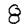
\includegraphics[width=\textwidth]{figure/mnist1}
	\end{subfigure}
	\begin{subfigure}{.23\textwidth}
		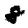
\includegraphics[width=\textwidth]{figure/mnist2}
	\end{subfigure}
	\begin{subfigure}{.23\textwidth}
		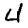
\includegraphics[width=\textwidth]{figure/mnist3}
	\end{subfigure}
	\begin{subfigure}{.23\textwidth}
		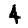
\includegraphics[width=\textwidth]{figure/mnist4}
	\end{subfigure}
	\caption{Training samples from the MNIST dataset that show the difficulty of achieving high classification accuracies.}
	\label{fig:mnist}
\end{figure}

We evaluate our neural net's performance on the Mixed National Institute of Standards and Technology (MNIST) dataset of handwritten digits \cite{mnist} in terms of overall training algorithm, network structure, number of filters, size of filters, number of pooling regions, and output layer activation function. The MNIST dataset contains 60,000 training images and 10,000 testing images. Its name comes from the NIST dataset that it is an adaptation of. In the NIST dataset, training and testing images were taken from two different sources, while in MNIST, the sources are merged. Each MNIST image contains a single handwritten digit (from zero to nine). The images are all 28 pixels by 28 pixels and grayscale. Figure \ref{fig:mnist} shows four training samples, two 4 digits and two 8 digits; since digits can be written in multiple ways and at different angles and sizes, classification is a difficult problem.

For our experimentation, we use a basic default setting of the neural network, and then adjust network parameters to identify patterns in the change in performance, such as test error rate and average per-iteration runtime. Specifically, we use a default setting of 64 filters, each 13 by 13, with a pooling layer of size 2 by 2 (meaning we have four pooling blocks, each pooling over an 8 by 8 region of the convolution output). The output from the pooling stage, then, consists of 256 values, which are fully connected to a final output layer consisting of ten neurons (without additional hidden layers in between); each neuron corresponds to one digit, and the maximum value over the neurons is the classification output.

\section{CNN Evaluation}

In this section, we show and analyze CNN performance under various network parameters tested in our experiment. Each parameter takes the default value in Table \ref{table:evaldefault} when unspecified in the subsections below.

\begin{table}
\begin{center}
\begin{tabular}{| c | c | c |}
\hline
Parameter & Value \\
\hline \hline
Filter sidelength $n$ & 13 \\
\hline
Number of filters $k$ & 64 \\
\hline
Pooling blocks & 2 by 2 \\
\hline
Output layer activation & Softmax \\
\hline
Training algorithm & SGD \\
\hline
Training duration & 10 hours \\
\hline
\end{tabular}
\end{center}
\caption{Default parameter values used for performance evaluation.}
\label{table:evaldefault}
\end{table}

\subsection{CNN performance under different network configurations}

To start, we explore how different configurations of the neural network after the convolution and pooling layers affect the performance of our CNN. For each configuration, we trained the network with the 60,000 training samples, and then tested on the 10,000 test samples from MNIST dataset. In each case we train the network for 10 hours.

Table \ref{table:change_in_neurons_in_hidden_layer} shows that iteration time remains mostly the same. As we go down the table, the model gets more complex, and the test error first goes down and then goes up, suggesting overfitting for the last model.

\begin{table}
\begin{center}
\begin{tabular}{| c | c | c |}
\hline
Hidden layer & Test & Time for one \\
configuration & error & iteration (sec) \\
\hline \hline
No hidden layer & 2.69\% & 30.48 \\
\hline
10-neuron hidden layer & 1.73\% & 30.80 \\
\hline
16-neuron hidden layer & 1.74\% & 30.66 \\
\hline
32-neuron hidden layer & 1.81\% & 30.56 \\
\hline
32-neuron followed by & 1.93\% & 30.43 \\
16-neuron hidden layers & & \\
\hline
\end{tabular}
\end{center}
\caption{Test error and per-iteration runtime for CNN training with various network configurations.}
\label{table:change_in_neurons_in_hidden_layer}
\end{table}

\subsection{Performance with variable filter size}

We next investigate how filter size affects the performance of our neural network. We tried out various filter sizes ranging from $n = 5$ to $n = 15$ (for filter sidelength $n$), again training for ten hours.

The results are shown in Figures \ref{fig:test_error_vs_filter_size} and \ref{fig:iter_time_vs_filter_size}. The horizontal axis of both figures show the filter size. For instance, when the filter size is ``7 by 7'', it achieves an test error rate at about 3.5\% and average iteration time takes about 20 seconds.

From the results, we can see that as filter size increases, the average iteration time generally increases. This is probably because low filter size model has fewer number of features, and the update of the features is faster. On the other hand, high filter size model has much more number of features. For instance, the ``15 by 15'' filter size model has 25 times many features than the ``5 by 5'' filter size model, and thus the update is much slower, which contributes to slower running time per iteration. From our experiment, the filter size that achieves the fastest running time is ``5 by 5'', the smallest of all filter sizes.

The test error rate generally decreases and then increases. This is probably because a very low filter size has too few features, and thus cannot capture all the information from the image; while a very high filter size tends to have too many features, and thus tends to overfit the training data and, as a consequence, performs badly in test data. Another problem with high filter size model is that the training time takes longer due to more features, and thus when terminated at a fixed time (as in our experiment), it will have run much fewer iterations then the low filter size model, i.e. the number of iteration completed is not sufficient. From our experiment, the optimal filter size range is from ``9 by 9'' to ``13 by 13''.

\begin{figure}
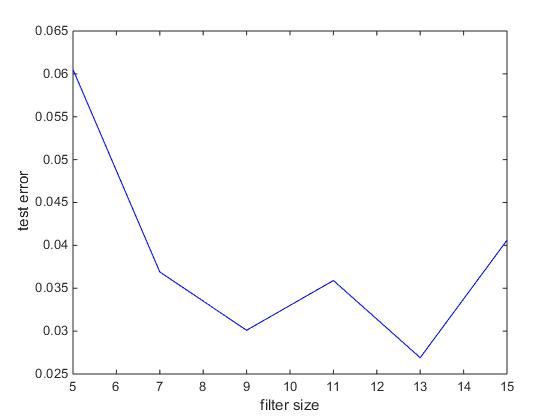
\includegraphics[width = 0.5\textwidth]{figure/test_error_vs_filter_size}
\caption{Test error against filter size.}
\label{fig:test_error_vs_filter_size}
\end{figure}

\begin{figure}
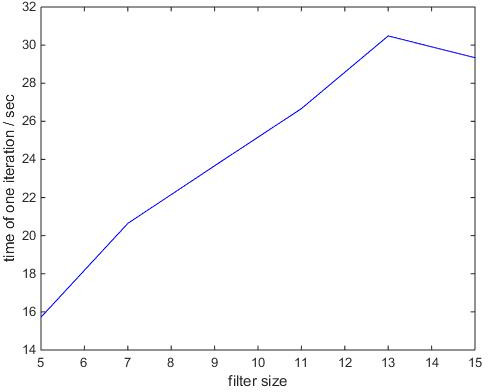
\includegraphics[width = 0.5\textwidth]{figure/iter_time_vs_filter_size}
\caption{Per-iteration runtime against filter size.}
\label{fig:iter_time_vs_filter_size}
\end{figure}

\subsection{Performance with variable filter count}

We then investigate how changing the number of filters affects CNN performance. Note that for all experiments in this subsection, we use the default setting of filter size ``13 by 13''. The number of filters we explored ranges from 8 to 256. Again, we train the network for each filter size for 10 hours.

The results are shown in Figures \ref{fig:test_error_vs_no_of_filters} and \ref{fig:iter_time_vs_no_of_filters}. The horizontal axis of both figures show the the number of filters used, and is plotted in log scales. For instance, when the number of filters is 16, it achieves an test error rate at about 3\% and average iteration time takes about 10 seconds.

From the results, we can see that as the number of filters increases, the average iteration time generally increases, with almost the same speed. This is as expected, because the fewer number of filters in the model, the less complex the model is, and hence the fewer parameters the model needs to update. For instance, the model that with 256 filters have approximately 16 times more parameters (weights, features, etc.) to update compared to the model with 16 filters, and this shows in Figure \ref{fig:iter_time_vs_no_of_filters} as the running time per iteration for the former model is about 16 times of that of the latter model.

The test error rate generally decreases and then increases. This is probably due to the same reason that we mention previously: models with low number of filters underfit the training data, while models with high number of filters tends to overfit. From our experiment, the optimal number of filters to use ranges approximately from 16 to 64.

\begin{figure}
\centering
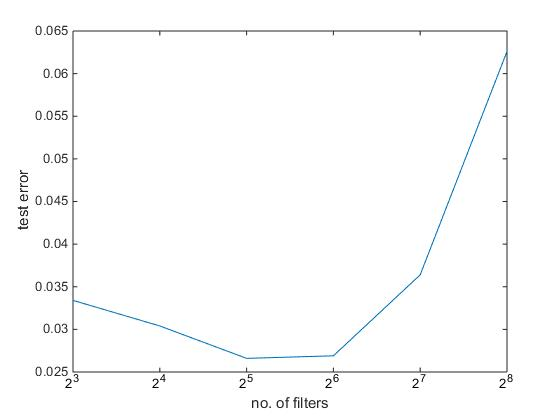
\includegraphics[width = 0.5\textwidth]{figure/test_error_vs_no_of_filters}
\caption{Test error against number of filters.}
\label{fig:test_error_vs_no_of_filters}
\end{figure}

\begin{figure}
\centering
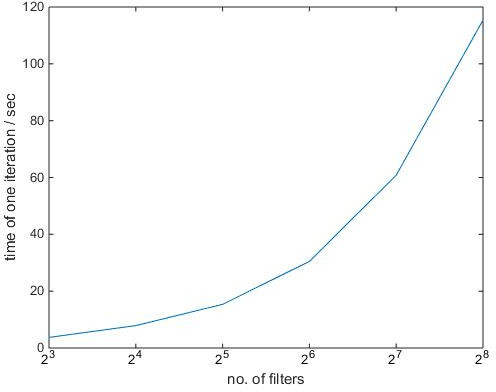
\includegraphics[width = 0.5\textwidth]{figure/iter_time_vs_no_of_filters}
\caption{Per-iteration runtime against number of filters.}
\label{fig:iter_time_vs_no_of_filters}
\end{figure}

\subsection{Performance with variable pooling size}

Next we investigate how different pooling sizes affect performance. The number of filters we explored ranges from the extreme case ``1 by 1'' (a single pooling block that averages over the entire output matrix from the convolution operation) to ``6 by 6''.

The results are shown in Figures \ref{fig:test_error_vs_pooling_size} and \ref{fig:iter_time_vs_pooling_size}. The horizontal axis of both figures show the the dimension of the pooling size used. For instance, when the pooling size is 4 by 4, it achieves a test error rate at about 4.2\% and average iteration time takes about 34 seconds.

From the results, we can see that as the number of pooling size increases, the average iteration time generally increases, with an almost linear relationship. This is as expected, because the fewer number of pooling blocks in the model, the less complex the model is, and hence the fewer parameters the model needs to update. For instance, the model that with pooling sizes of ``6 by 6'' have many more parameters (specifically weight and bias terms between the pooling layer and the output layer, which are fully connected) to update compared to the model with pooling size ``1 by 1'', and this shows up in Figure \ref{fig:iter_time_vs_pooling_size}.

Again, the test error rate shows a ``U-shape'' trend, and the reason is similar to that in the previous subsection: models with low number of pooling blocks underfit the training data, while models with high number of pooling blocks tend to overfit. From our experiment, the optimal pooling size is ``2 by 2''.

\begin{figure}
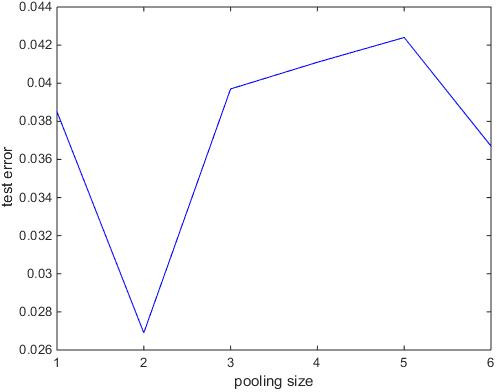
\includegraphics[width = 0.5\textwidth]{figure/test_error_vs_pooling_size}
\caption{Test error against pooling size.}
\label{fig:test_error_vs_pooling_size}
\end{figure}

\begin{figure}
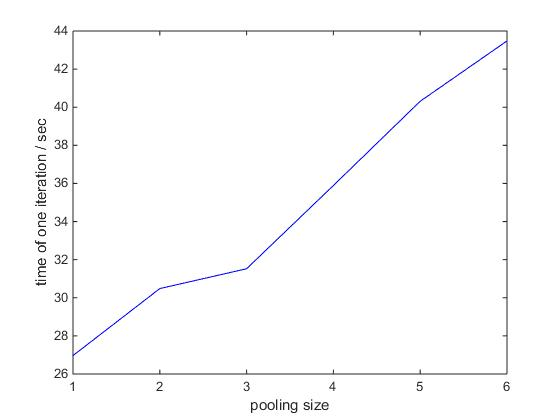
\includegraphics[width = 0.5\textwidth]{figure/iter_time_vs_pooling_size}
\caption{Per-iteration runtime against pooling size.}
\label{fig:iter_time_vs_pooling_size}
\end{figure}

\subsection{Other parameters}

We also experiment with using sigmoid activation function in the output layer (instead of the default softmax activation function used over the other experiments), and training with conventional gradient descent rather than stochastic gradient descent (SGD).

Softmax activation resulted in an error rate of 59.62\% compared to 2.69\% with the default settings for softmax activation function. This indicates that the cross-entropy cost function is critical to training convolutional neural networks for multi-label classification, otherwise multiple neurons might fire and the cost does not take into account differentiating between the size of the activation outputs.

Gradient descent only completed five iterations in the ten hours allocated for training, and got an error rate of 90.2\%. This is equivalent to a random classifier, so clearly the network was not trained for long enough to have a useful structure. Stochastic gradient descent, which achieved the 2.69\% error, solves this problem by randomly taking subsets of the data during each iteration so that we can train for a higher number of iterations, even if there is greater variance in the derivatives at each iteration.

\begin{figure}
\centering
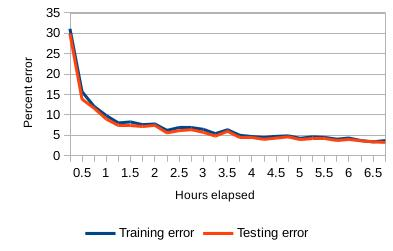
\includegraphics[width = 0.5\textwidth]{figure/error_over_time}
\caption{Training and testing error at different training durations (plotted at fifteen minute intervals).}
\label{fig:error_over_time}
\end{figure}

Figure \ref{fig:error_over_time} shows percent classification error on the training and testing datasets as the CNN training algorithm progresses. At the beginning, the improvement is much more significant, while later on we approach the best solution and are no longer able to make significant gains; in the later three hours shown, we only decrease the error rate by an additional few percentage points. Also, as a result of the stochastic gradient algorithm (which updates based on random samples at each iteration), the training error is not monotonically decreasing.

\begin{figure}
	\centering
	\begin{subfigure}{.23\textwidth}
		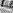
\includegraphics[width=\textwidth]{figure/filter1}
	\end{subfigure}
	\begin{subfigure}{.23\textwidth}
		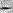
\includegraphics[width=\textwidth]{figure/filter2}
	\end{subfigure}
	\caption{Examples of convolutional filters. These filters are 13 by 13 pixels.}
	\label{fig:filter}
\end{figure}

Figure \ref{fig:filter} shows two example convolutional filters after training. It appears that these filters recognize parts of digits; the output layer weights can then take care of piecing the parts together to recognize the entire handwritten digit.

\subsection{Heatmap}

\section{Comparison with HOG-feature recognition} \label{sec:evalfeature}

Before deep learning techniques became widely used in image recognition, various other methods were used to extract the features from the image and models were trained on these features. Examples include histogram of oriented gradients (HOG) and scale-invariant feature transform (SIFT). In this section, we will compare the performance of our CNN implementation with the performance of using HOG with SVM classifier, using different percentages of the 60,000 training samples. We use the default parameters except we include a ten-neuron fully connected hidden layer between the pooling and output layers.

We implemented the CNN library for this project, but we used MATLAB packages for the HOG feature extraction method. HOG divides an image into cells and computes a local histogram of gradient orientations in each cell. The histograms and normalized and grouped across block regions, and these descriptor values can then be fed into a classifier.

The results are shown in Figures \ref{fig:hog} and \ref{fig:neural_net_percentage_data}. From the figures, we can see that the training error rate is generally lower than the testing error rate, and this is expected because our model is based on the training set. Moreover, as we use more training data, we generally get a higher training error, but a lower testing error. This is because with less training data, it is much easier to fit a model that does very well on the training set, but the same model does not generalize well to the overall data, and thus performs badly on the testing set. As the training set data increases, although we get a higher training error as it becomes increasingly harder to fit a perfect model on the training set, the testing error generally decreases. This agrees with our intuition.

Moreover, we can see that our CNN performs much better than the HOG feature-extraction technique. At any percentage of training data, our model achieves a test error strictly less than the HOG feature-extraction technique. When all training data is used, our neural net model achieves an error rate of about 2.25 percent test error, while the HOG feature-extraction technique achieves more than 5 percent. This perhaps explains why the old feature-extraction techniques, such as HOG and SIFT, are becoming increasingly obsolete today, due to the advent of deep learning.

\begin{figure}
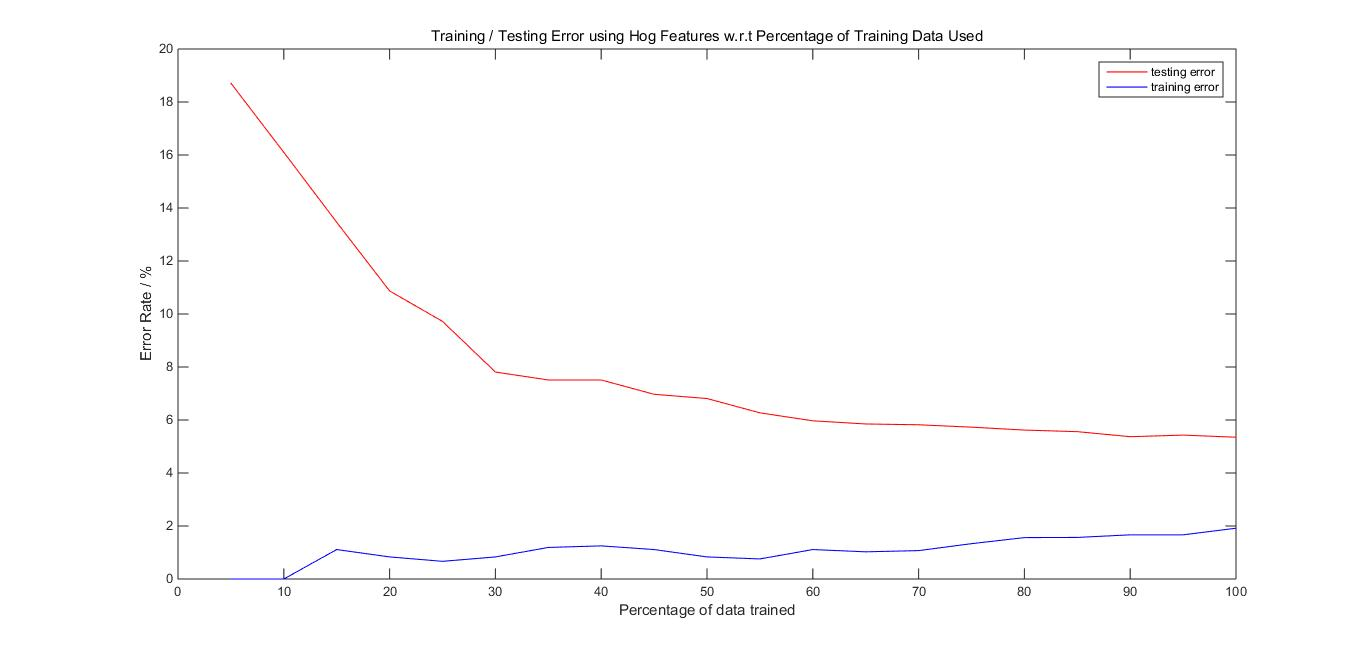
\includegraphics[width = 0.5\textwidth]{figure/hog}
\caption{Training and testing error using HOG features against percentage of training data used.}
\label{fig:hog}
\end{figure}

\begin{figure}
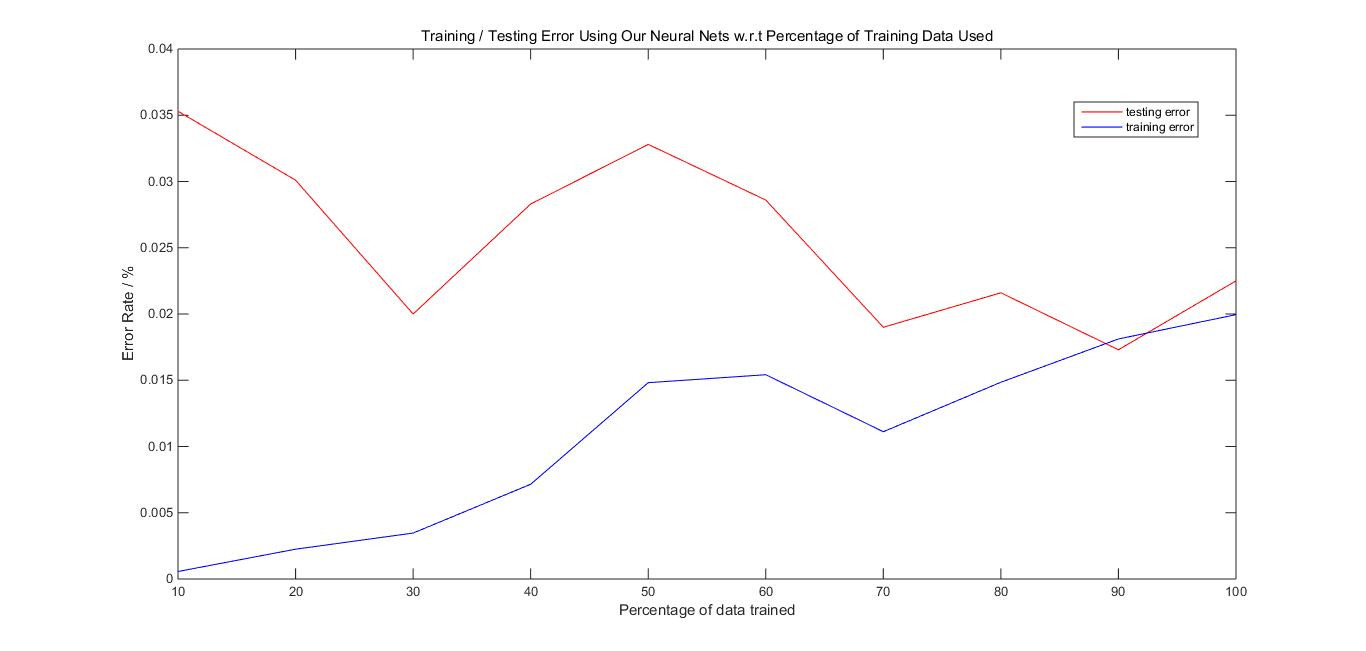
\includegraphics[width = 0.5\textwidth]{figure/neural_net_percentage_data}
\caption{Training and testing error of CNN against percentage of training data used.}
\label{fig:neural_net_percentage_data}
\end{figure}

\section{Conclusion} \label{sec:conclude}

With our basic CPU-based Python convolutional neural network toolkit, we are able to achieve error rates as low as 1.73\% for certain network parameter choices. Deep learning algorithms like CNNs allow machine learning of the very features to be used for classification; this contrasts with previous approaches where feature functions are designed by humans. CNNs show that biologically inspired machine learning algorithms often can improve performance; this echoes previous work in genetic algorithms and ant colony optimization.

However, CNN training did take significantly longer than feature extraction and SVM classification. Still, GPU-based CNN libraries take advantage of parallelizable sequences of matrix operations that perform very well on modern GPUs. Additionally, optimizations can be made when using stochastic gradient descent for the batch size.

There were also cases where we used a CNN that was too complex (too many filters or too many network layers) and resulted in overfitting. There has been significant research in preventing CNN overfitting. One approach called ``dropout'' randomly disables half of the filters on each training iteration and yields promising performance \cite{dropout}.

\section{Appendix: Sample Code}

\subsection{Implementation of the Neural Net}

\bibliography{report}{}
\bibliographystyle{plain}

\end{document}
